\documentclass{anstrans}
%%%%%%%%%%%%%%%%%%%%%%%%%%%%%%%%%%%
\title{Evidence of the necessity of isotopic precise calculation in fuel cycle
calculation}
\author{ Baptiste Mouginot$^{*}$, Paul P.H. Wilson$^{*}$, Robert W. Carlsen$^{*}$ }

\institute{
$^{*}$University of Wisconsin-Madison, WI
}

\email{mouginot@wisc.edu \and paul.wilson@wisc.edu}

% Optional disclaimer: remove this command to hide
%\disclaimer{Notice: this manuscript is a work of fiction. Any resemblance to
%actual articles, living or dead, is purely coincidental.}

%%%% packages and definitions (optional)
\usepackage{graphicx} % allows inclusion of graphics
\usepackage{booktabs} % nice rules (thick lines) for tables
\usepackage{microtype} % improves typography for PDF

\newcommand{\SN}{S$_N$}
\renewcommand{\vec}[1]{\bm{#1}} %vector is bold italic
\newcommand{\vd}{\bm{\cdot}} % slightly bold vector dot
\newcommand{\grad}{\vec{\nabla}} % gradient
\newcommand{\ud}{\mathop{}\!\mathrm{d}} % upright derivative symbol

\begin{document}
%%%%%%%%%%%%%%%%%%%%%%%%%%%%%%%%%%%%%%%%%%%%%%%%%%%%%%%%%%%%%%%%%%%%%%%%%%%%%%%%
\section{Introduction} 

The purpose of this study is to examine the importance of the isotopic
composition of plutonium on PWR MOX fuel fabrication as part of a multi-tiered
fuel cycle, and the effect of its evolution during a transition. Two main
effects can modify the isotopic composition of the plutonium used to build the
PWR-MOX fuel: decay and depletion.

This analysis is based on a transition of the nuclear fuel cycle
to a configuration identified as ``Evaluation Group 29'' or ``EG29'', in the
recently-published Evaluation and Screening (E\&S) report \cite{ES}.  The EG29 fuel
cycle corresponds to a double strata fleet. The first stratum is composed of
sodium-cooled fast reactors (SFRs) multi-recycling plutonium. Surplus
plutonium is sent to the second stratum composed of pressurized water
reactors with full mixed oxide (U/Pu)O$_{2}$ cores (MOX-PWRs).  The PWR stratum
is also multi-recycling its plutonium. The target energy generation ratio for
the final EG29 system is 70:30 (SFR:PWR), with a 1\% annual growth in nuclear
energy demand.

\begin{figure}[ht] % replace 't' with 'b' to force it to be on the bottom
  \centering
  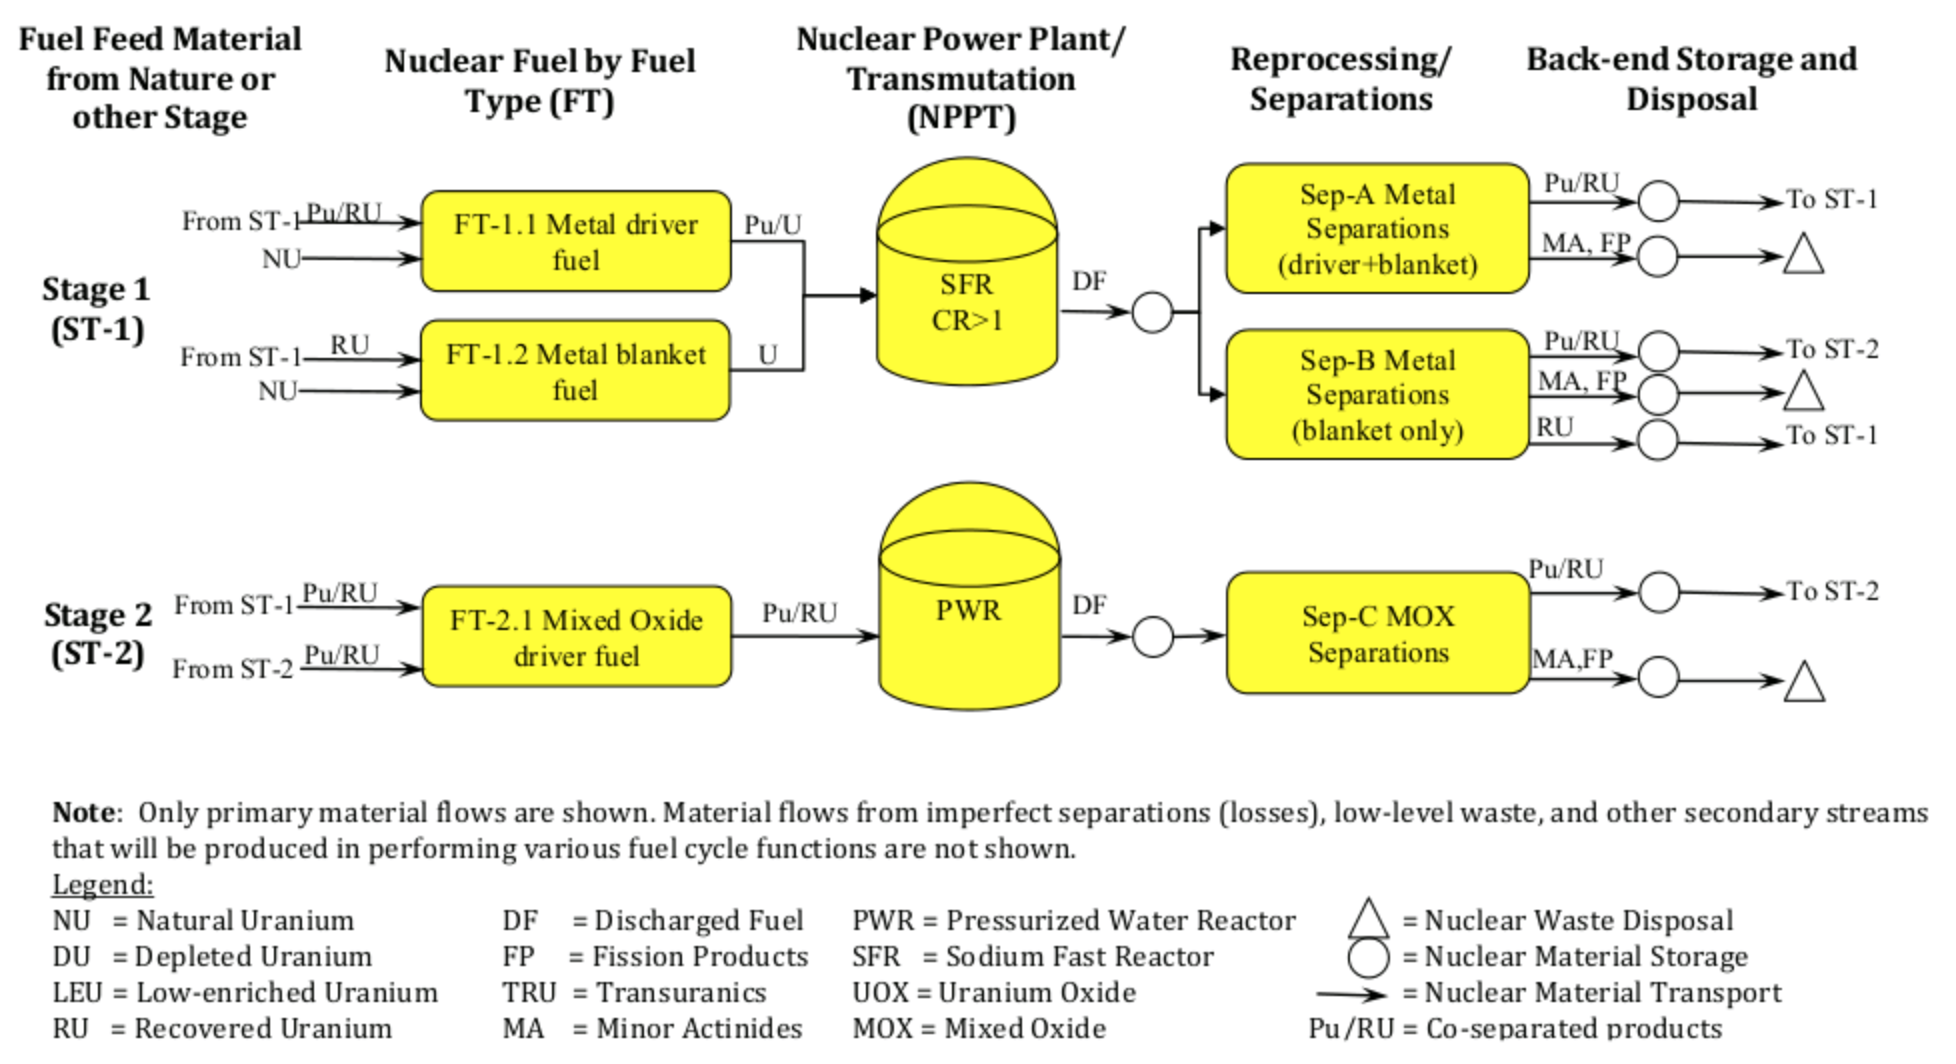
\includegraphics[width=0.48\textwidth]{FCDP_cycle}
  \caption{Schematic representation of the EG29 fuel cycle taken from \cite{FCDP}.}
  \label{fig:FCDP}
\end{figure}
%% PPHW: Can we add the official FCDP images

All the calculation of this study have been performed using the Cyclus fuel cycle
tool\cite{CYCLUS}. The facility models are from the Cycamore package, developed by the
Cyclus team, and containing a Pu-equivalent fuel fabrication model as well as
a simple fixed mixing ratio fuel fabrication model. A new neural network model has
also been contributed to the Cyclus environment using the cyCLASS tool\cite{cyCLASS}, 
allowing the use of the fuel fabrication and depletion models from the CLASS tool
\cite{CLASS} in Cyclus.


\section{Study description}

This work compares the plutonium fraction required to build fresh MOX fuel
using three different stream mixing models in fuel fabrication: ``fixed mixing
ratio'', ``plutonium equivalent theory'', ``neural network'' \cite{Leniau2015125}.
The first part of the study in focuses on the effect of decay on the isotopic
composition of the reprocessed plutonium and its impact on fuel fabrication
depending on the chosen stream mixing model.  The second part of the study,
compares the impact on fresh fuel compositions when used fuel is based on a
depletion calculation instead of a fixed recipe, using the neural network fuel
fabrication model, also including the impact of decay.


\subsection{Cycle}

This analysis is focused only on the second strata of EG29, represented by a
single PWR reactor using MOX fuel. After irradiation the uranium and the
plutonium are separated and reprocessed to fuel the next batch of MOX fuel for
the PWR. The separation efficiency is $0.988$. The separated U/Pu (``J1''
stream) is then separated into two sub-stream, one used for new PWR deployment
(``J1\_prime\_storage'' on Fig. \ref{fig:flow}) and the other one for the
production the new batch of MOX fuel (``J1\_second\_storage''). The respective
fraction of those sub-stream are $0.105$ and $0.895$.

\begin{figure}[ht] % replace 't' with 'b' to force it to be on the bottom
  \centering
  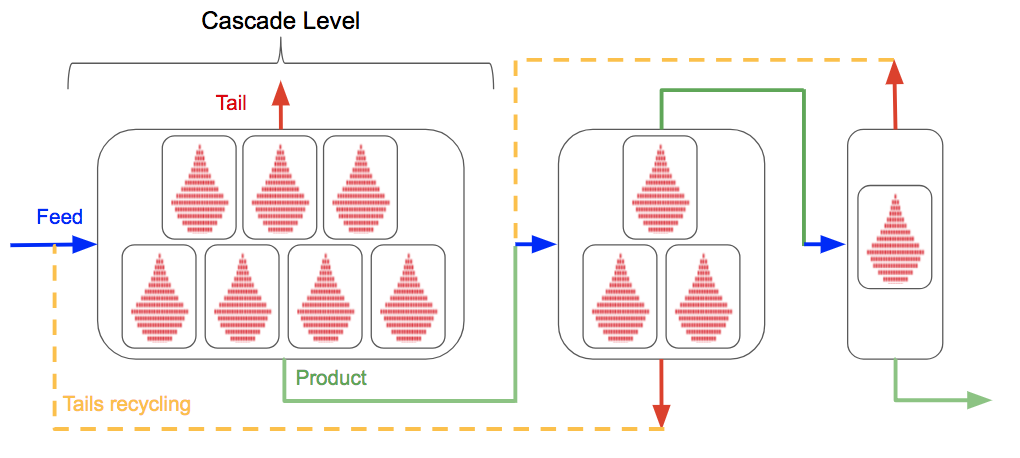
\includegraphics[width=0.48\textwidth]{flow}
  \caption{Schematic representation of the fuel cycle. Quantities on the row
  represents the cumulative amount in kg of material exchanged between two
  facilities in the calculation using ``pu-equivalent'' for fuel fabrication
  modeling with decay activated.}
  \label{fig:flow}
\end{figure}

A stream (``E3'') of ``good'' quality plutonium coming from a hypothetical irradiated
SFR blanket is represented by a storage facility
(``E3\_second\_limited\_storage`` on Fig. \ref{fig:flow}).

\begin{table*}[htb]
  \centering
  \begin{tabular}{llllllllllll}\toprule
    Stream 
    & $^{234}$U   & $^{235}$U   & $^{236}$U   & $^{238}$U   
    & $^{238}$Pu  & $^{239}$Pu  & $^{240}$Pu  & $^{241}$Pu  & $^{242}$Pu 
    & $^{241}$Am  & F.P. \\ \midrule
    E3 [\%]
    & $0.002$   & $0.203$    & $0.083$   & $81.082$
    & $0.0087$  & $17.9764$  & $0.6166$  & $0.0216$  & $0.0007$
    & $0$         & $0$ \\
    J1 [\%]
    & $0$       & $0$        & $0$       & $93.632$
    & $0.1216$  & $2.7058$   & $1.8193$  & $0.7402$  & $0.6833$
    & $0.2978$  & $0$ \\
    \bottomrule
  \end{tabular}
  \caption{Streams compositions in percentage by mass.}
  \label{tab:strem_compo}
\end{table*}

The impact of the decay on this stored Pu is limited, as the content in
$^{241}$Pu is almost negligible (see Tab. \ref{tab:stream_compo}).  
 
In order to build the first batches of fuel, an initial quantity of 225t has
also been provided in the ``J1\_second\_storage'', which corresponds to 3 times
the requirement on ``J1'' stream to build the PWR-MOX fuel for full PWR
core. 




\subsection{Fabrication model}
Three different ways to model the fuel fabrication have been used: ``fix mixing
ratio'', ``Pu-equivalent'' and ``neural network''.
The fix mixing ratio is based on a user-defined ratio for the J1 and E3 stream
mixing. The respective mixing ratio used for J1 and E3 stream are 
$0.8357$ and $0.1643$.
The ``Pu-equivalent'' model finds the mixing ratio that results in an initial
reactivity that matches that of the requested MOX fuel recipe.  This ratio may
change as the composition of the incoming streams changes.  As the requested
fuel composition corresponds to the fuel composition built with the ''fix mixing
ratio`` model, the results of those 2 models are expected to be similar.  The
``neural network'' model attempts to achieve a given reactivity at the  end of
cycle reactivity of the whole core for a multi-batch core ($50~$GWd/t in this
study). The $k_{infty}$ used in this study is 1.034, assuming the reactivity of
the full core is the mean reactivity of the batches. The neural network in this
model has been pre-trained on several different depletion calculations, allowing
it to predict the correct plutonium fraction required, depending on the
composition of that plutonium.

Because the neural network model allows only to mix a plutonium stream into a
uranium stream, slight modification have been made on the cycle: in both ``J1''
and ``E3'' streams uranium and plutonium are separated, the uranium and
plutonium sub-streams are mix together to build one stream of pure uranium and
one stream of pure plutonium. That is why, when comparing the different fuel
fabrication models only the total plutonium enrichement are compared. 

Because of these models have not necessary been tuned on exactly the same
PWR configuration and parameters, this analysis focuses on the differences
in the results due to the change in model rather than the results themselves.

The second part of the study compares the amount of plutonium require to build
the PWR-MOX fuel (using the neural network modeling for fuel fabrication) for
the recipe based output composition versus a composition calculated by
depletion.  To calculate the depletion for each fuel batch loaded in the PWR
reactor, another neural network is used to predict the macroscopic cross section
of the fuel \cite{Leniau2015125} (only fission, capture and n,2n reactions are
considered). The depletion calculation is done renormalizing the neutron flux to
maintain a constant power in the reactor.

%%%%%%%%%%%%%%%%%%%%%%%%%%%%%%%%%%%%%%%%%%%%%%%%%%%%%%%%%%%%%%%%%%%%%%%%%%%%%%%%
\section{Decay}


As observed in Fig. \ref{fig:nod}, despite the fact that the different models
were not tuned to describe the exact same PWR concept, the results without decay
are very close. They all predict a constant plutonium fraction around $8\%$ of
plutonium in the fresh PWR-MOX fuel.

\begin{figure}[ht] % replace 't' with 'b' to force it to be on the bottom
  \centering
  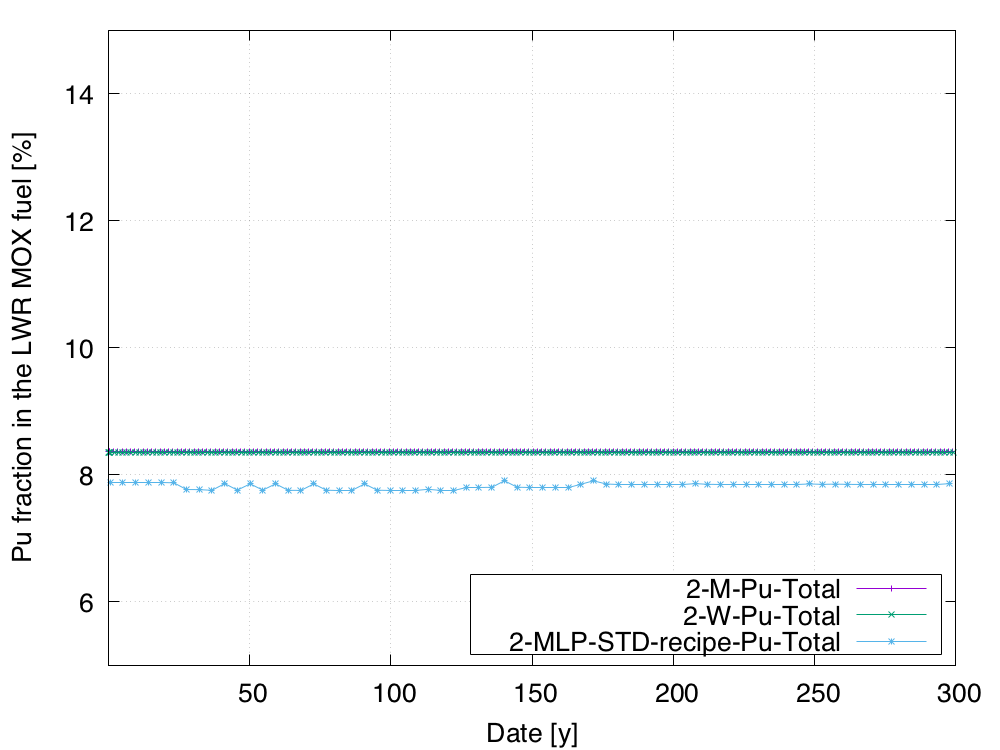
\includegraphics[width=0.48\textwidth]{nodecay_pu_contribution.png}
  \caption{Evolution of the fraction of plutonium in the fresh PWR-MOX fuel
  using the 3 predicted models: ``fix mixing ratio'' (``fix'', blue), ``Pu-equivalent''
  (``Pu-eq'', green) and ``Neural Network'' (``NN'', red), without considering decay.}
  \label{fig:nod}
\end{figure}

With decay turned on, see Fig. \ref{fig:d}, results for the ``fix mixing ratio''
calculation see a small decrease of the fraction of plutonium in the fuel,
corresponding to the decay of $^{241}$Pu into $^{241}$Am.  For the
``Pu-equivalent'' modeling we can observe a slight increase of the fraction of
plutonium, which is required to compensate for the negative reactivity effect
coming from the $^{241}$Am. For the calculation using ``neural network'' fuel
fabrication modeling the effect is very quickly increasing to $13\%$ and then
slowing stabilizing as the plutonium composition approaches an equilibrium.

\begin{figure}[h!] % replace 't' with 'b' to force it to be on the bottom
  \centering
  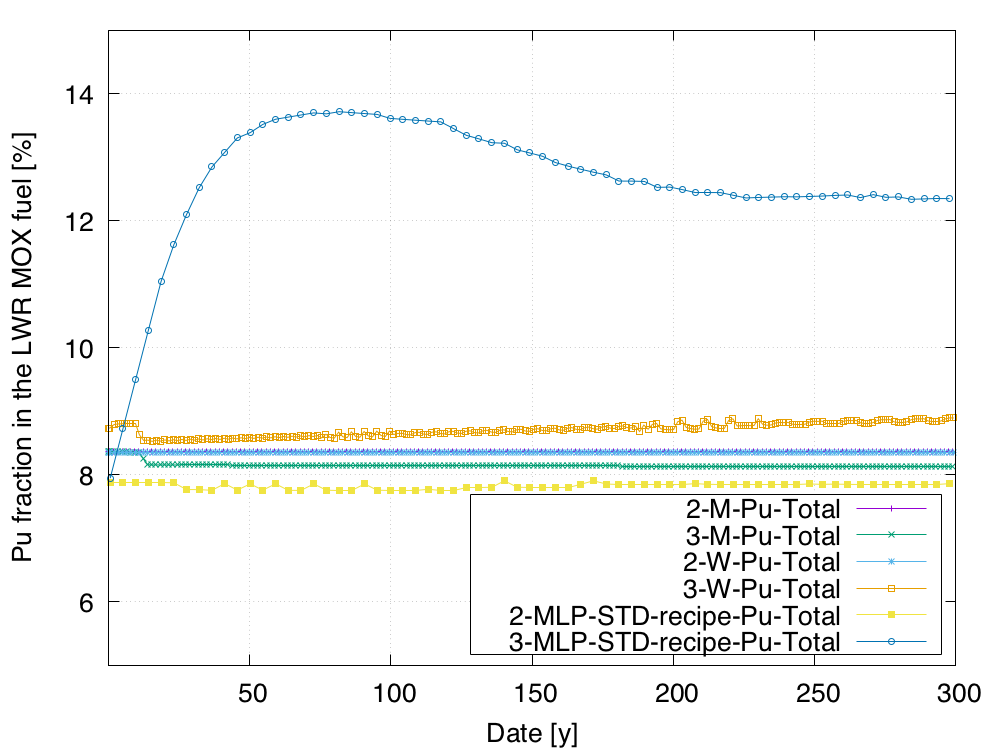
\includegraphics[width=0.48\textwidth]{decay_pu_contribution.png}
  \caption{Evolution of the fraction of plutonium in the fresh PWR-MOX fuel
    using the 3 prediction models: ``fix mixing ratio'' (``fix'', blue),
    ``Pu-equivalent'' (``Pu-eq'', green) and ``Neural Network'' (``NN'', red),
    with (solid line) and without (dash line) decay enable.} 
  \label{fig:d}
\end{figure}


As the calculation using ``neural network'' fabrication modeling requires more
plutonium than the cycle can produce, the initial inventory has been set to a
higher values, increasing the plutonium decay effect. Nevertheless this shows
the strong impact of the presence of $^{241}$Am with the plutonium used for the
PWR-MOX fuel fabrication.

%% PPHW: why is the Pu-equiavlent model so bad?

A last calculation, on decay have been performed using the ``Pu-equivalent''
fabrication model, increasing by a factor 2, 5 and 10 the amount of plutonium in
the startup inventory. This mimics different degrees of a plutonium accumulation,
and thus different impacts from the decay of this plutonium.
This calculation results in a change in the mixing ratio required to build the
PWR-MOX fuel of 10 to 30\%. This kind of plutonium accumulation can
unexpectedly occur in a real fuel cycle and might need to be considered in a
complete fuel cycle transition study.


The decay process tends to change to composition of the plutonium vector, and
then of the plutonium enrichment required to build a proper PWR-MOX fuel.  Such
composition change in the MOX fuel will impact the individual cross sections:
particularly in thermal reactors where the macroscopic cross sections are very
dependent on the shape of the thermal part of the neutron spectrum, which is
strongly driven by the fuel isotopic composition.


%%%%%%%%%%%%%%%%%%%%%%%%%%%%%%%%%%%%%%%%%%%%%%%%%%%%%%%%%%%%%%%%%%%%%%%%%%%%%%%%
\section{Depletion vs Recipe}

Another analysis was performed to evaluate the impact of the depletion
calculation on a fuel cycle macroscopic (???) level.

\begin{figure}[ht] % replace 't' with 'b' to force it to be on the bottom
  \centering
  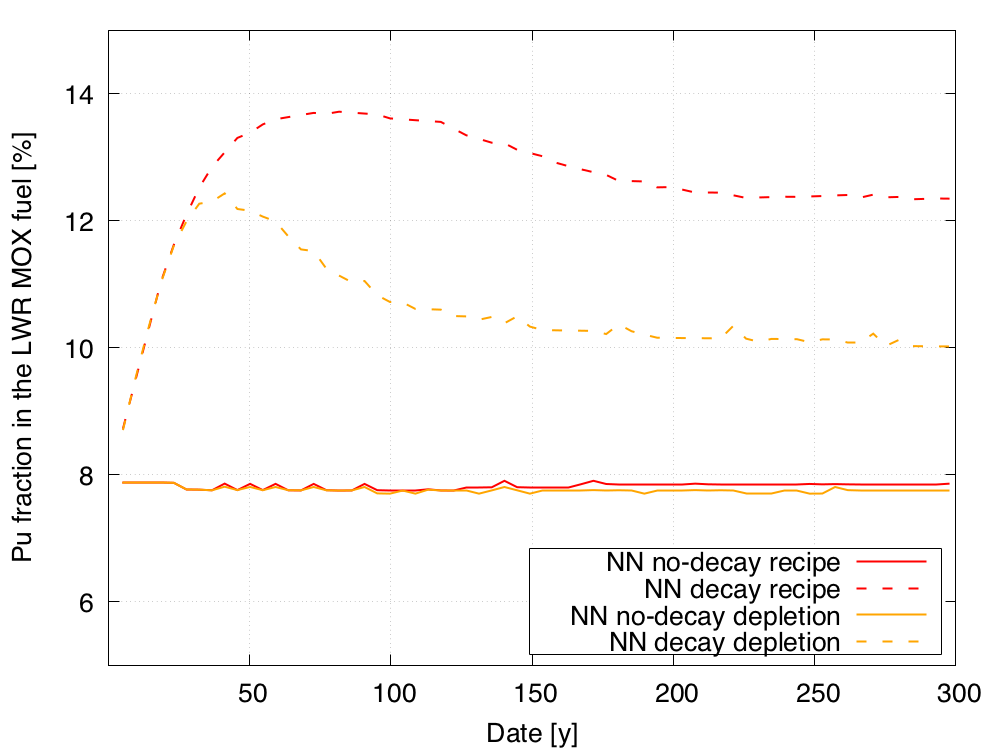
\includegraphics[width=0.48\textwidth]{irradiation_pu_contribution.png}
  \caption{Evolution of the fraction of plutonium in the fresh PWR-MOX fuel
    using the ``Neural Network'' prediction models, using recipe based spent
    fuel composition (red) and recalculated spent fuel composition (orange),
    with (solid line) and without (dash line) decay enable.}
  \label{fig:depletion}
\end{figure}


Four simulations were carried out representing variations across two problem
dimensions.  One variation compares how reactor models determine the recipe of
used fuel.  The standard recipe reactor model produces used fuel of a fixed
composition, regardless of the composition of the incoming fuel.  The
alternative is a neural network depletion model provided by the cyCLASS
package.  This model determines the composition of the used fuel depending on
its initial composition and discharge burnup.  Both of these models were used
without decay and with decay.

As shown on Fig. \ref{fig:depletion}, the equilibrium values for recipe based
calculation and the depletion calculation are not the same. Moreover,
recalculating the fuel spent fuel composition for each fuel batch allows the
cycle to reach equilibrium faster.

This is caused by the slight change in the composition in the available
plutonium (see Fig. \ref{fig:depletioncompo}): in the case of the depletion
calculation the available plutonium contain $68\%$ of $^{239}$Pu versus $64\%$
in the recipe based case, and also less $^{242}$Pu and $^{241}$Am, respectively
$4.8\%$ and $5.4\%$ in the depletion case versus $7.3\%$ and $6.7\%$. The
amounts of the other nuclides are very close.


\begin{figure}[ht] % replace 't' with 'b' to force it to be on the bottom
  \centering
  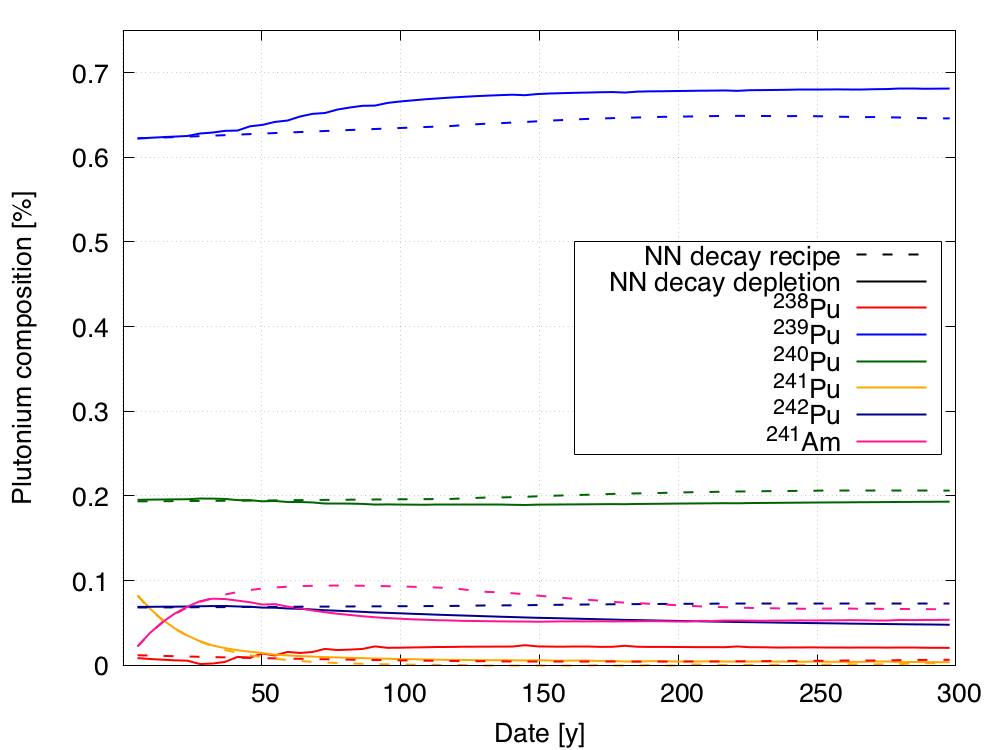
\includegraphics[width=0.48\textwidth]{MOX_pu_composition.png}
  \caption{Evolution of the composition of the plutonium in the fresh PWR-MOX fuel
  using the ``Neural Network'' prediction models, with decay enable using recipe
  based spent fuel composition (plain line) and recalculated spent fuel
  composition (dash line).}
  \label{fig:depletioncompo}
\end{figure}

Those slight change in the output composition, lead to an overall decrease in
the amount of $^{241}$Am in the fresh PWR-MOX fuel and an increase of the
$^{239}$Pu, allowing to build fuel with a lower plutonium enrichment.


%%%%%%%%%%%%%%%%%%%%%%%%%%%%%%%%%%%%%%%%%%%%%%%%%%%%%%%%%%%%%%%%%%%%%%%%%%%%%%%%
\section{Conclusions}

This study has shown the potential impact of the decay process on the MOX-PWR fuel
fabrication process, increasing the required amount from $1\%$ to $4\%$
depending on the fuel fabrication model choice. The recalculation of the 
depletion of each loaded fuel batch has consequences on the equilibrium
state of the calculation: the reduction of fraction of $^{241}$Am and the increase of the
fraction $^{239}$Pu in the available plutonium allows a reduction in the amount of
plutonium in the fuel.

This work has shown the strong influence of the isotopic composition on a LWR
cycle involving plutonium recycling. Similar analysis will be conducted in the
near future on the SFR strata of the EG29 fuel cycle, which should be less
impacted by those isotopic changes, as fast spectrum reactor are less sensitive
to those change.

Moreover this study has demonstrated the value of the modular design of
Cyclus, able to investigate differences between the physics fidelity of
facility models in an isolated fashion, with other fuel cycle components
unchanged.  In this case, additional fidelity was introduced rapidly by
wrapping the existing neural network models made available by CLASS.



%%%%%%%%%%%%%%%%%%%%%%%%%%%%%%%%%%%%%%%%%%%%%%%%%%%%%%%%%%%%%%%%%%%%%%%%%%%%%%%%
%\appendix
%\section{Appendix}
%
%Numbering in the appendix is different:
%\begin{equation} \label{eq:appendix}
%  2 + 2 = 5\,.
%\end{equation}
%and another equation:
%\begin{equation} \label{eq:appendix2}
%  a + b = c\,.
%\end{equation}

%%%%%%%%%%%%%%%%%%%%%%%%%%%%%%%%%%%%%%%%%%%%%%%%%%%%%%%%%%%%%%%%%%%%%%%%%%%%%%%%
\section{Acknowledgments} 
This work was funded in part by the Nuclear Energy University Program 
(DE-NE0000673) and Idaho National Laboratory (154956).
\begin{center}

\includegraphics[width=1.5in]{neup_logo_large.jpg}
\end{center}

%%%%%%%%%%%%%%%%%%%%%%%%%%%%%%%%%%%%%%%%%%%%%%%%%%%%%%%%%%%%%%%%%%%%%%%%%%%%%%%%
\bibliographystyle{ans}
\bibliography{bibliography}
\end{document}

